\subsection{Single Flower}\label{p:single}

This problem is designed to have you create a node and generate specific behavior for your turtle
using \texttt{numpy} commands. Your turtle's objective is to create a single flower pattern. See
Figure~\ref{fig:1} for exactly what the flower should look like.

The work for this problem should be done in file \texttt{singleflower.py}. Look for the comments
throughout the code that correspond to the instructions in the writeup.

\begin{enumerate}[(a)]
  \item In \texttt{\_\_init\_\_}:
    \begin{enumerate}[i.]
      \item Start a new node with the name `flower'.
      \item Create a publisher that publishes to    \texttt{/turtle1/cmd\_vel} with type
        \texttt{Twist} and a queue size of $10$.
      \item Set your rate to $5$.
    \end{enumerate}
  \item In \texttt{draw\_flower}:
    \begin{enumerate}[i.]
      \item To calculate constants, use \texttt{numpy} to perform the following operations on the
        following matrices:

        $$M_1 = \begin{bmatrix} 
          1.5 & -1.5 & 0\\
          -1.5 & 0 & 2 \\
          2.5 & 0 & 0
        \end{bmatrix} 
        M_2 = \begin{bmatrix} 
          3 & 5 & 9\\
          -1 & 2 & 6 \\
          -3 & 2 & 0
        \end{bmatrix}$$
        $$a = (M_1*M_2)_{(0,1)}+ (M_1*M_2)_{(1,1)}$$
        $$b = -(\langle M_1, M_2 \rangle_{(0,2)} + \langle M_1, M_2 \rangle_{(1,2)}) -1$$
        $$A = \langle M_1, M_2 \rangle_{(0,1)} - \langle M_1, M_2 \rangle_{(0,0)} + 0.5$$
        $$B = -((M_2*M_1)_{(1,2)}-(M_2*M_1)_{(2,1)})$$
        $$\texttt{max\_times} = (\texttt{det}(M_2)/-9) - 4$$
        \textbf{Note}: Angle brackets indicate taking an inner product, subscripts indicate the
        indices of the term that should be taken from a matrix
      \item Each of the above computed constants should be set as rosparams \texttt{a}, \texttt{b},
        \texttt{A}, \texttt{B}, and \texttt{max\_times} with the type \texttt{float}.
      \item In \texttt{while not rospy.is\_shutdown()} section: Use \texttt{numpy} to set angular z
        to $B * \cos(b*count)$ and linear x to $A * \sin(a*count)$. Be sure to publish your velocity
        message and sleep your turtle for your preset rate.
      \item Also in \texttt{while not rospy.is\_shutdown()} section: If value $count$ is greater
        than $2*(\texttt{times})*\pi$:  publish a velocity message with angular $z=5$ and linear
        $x=0$, then increment \texttt{times} by 1 and if \texttt{times} is greater than
        \texttt{max\_times} stop drawing the flower.
    \end{enumerate}

  \item 
    In \texttt{if \_\_name\_\_ == `\_\_main\_\_'} section:

    Create your turtle and have the turtle use your written function to draw a flower. Your final
    product should look something like Figure~\ref{fig:1}.

    \begin{figure}[h]
      \centering
      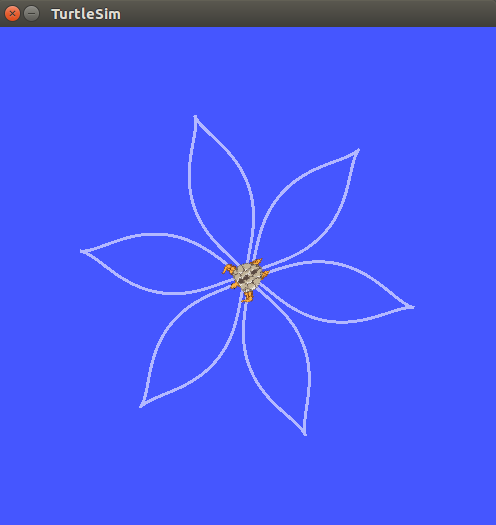
\includegraphics[width=150pt]{figures/p1/problem2.png}
      \caption{For Problem~\ref{p:single}. Single Flower}\label{fig:1}
    \end{figure}  
    %WOW omg replace this image with something more legit before release
  \item In \texttt{singleflower.launch}:
    \begin{enumerate}[i.]
      \item Launch the turtlesim node.
      \item Launch the \texttt{flower\_turtle} node from \texttt{singleflower.py}.
    \end{enumerate}
\end{enumerate}

%%% Local Variables:
%%% mode: latex
%%% TeX-master: "../assessment"
%%% End:
